\chapter{Philosophy of Science
科学哲学}\label{philosophy-of-science-ux79d1ux5b66ux54f2ux5b66}

\emph{这个部分整理者没什么好说的,只放一下关于这个概念的维基百科页面的机翻或其他相关的文章。}

\section{Self-reference 自指}\label{self-reference-ux81eaux6307}

\emph{Ascending and Descending} by M. C. Escher:

\begin{center}
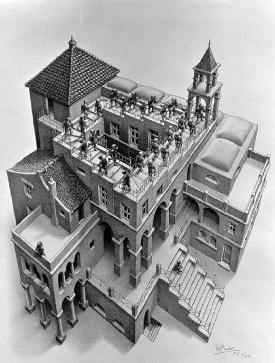
\includegraphics[height=200pt]{../assets/Ascending_and_Descending.jpg}
\captionof{figure}{Ascending and Descending}
\end{center}

Below is the Google translate of \textit{Wikipedia: Self-reference} (\url{https://en.wikipedia.org/w/index.php?title=Self-reference&oldid=1178832976}):

\begin{quote}
自我参照是一个涉及到自己或自己的属性、特征或行为的概念。
它可以发生在语言、逻辑、数学、哲学等领域。

在自然或形式语言中,当句子、想法或公式引用自身时,就会发生自引用。
引用可以直接表达------通过一些中间句子或公式------或者通过一些编码。

在哲学中,自我指涉也指主体能够讲述或指称自身的能力,即具有英语中第一人称单数主格代词``我''所表达的那种思想。

自我参照在数学、哲学、计算机编程、二阶控制论、语言学以及幽默中得到研究和应用。
自我指涉陈述有时是自相矛盾的,也可以被认为是递归的。

\textbf{逻辑、数学和计算}

在古典哲学中,悖论是由自我指涉的概念造成的,例如全能悖论,即询问是否有可能存在一个如此强大的存在,以至于它可以创造出一块它无法举起的石头。
埃皮米尼德悖论``所有克里特岛人都是骗子'',由古希腊克里特岛人说出,是最早有记录的版本之一。
当代哲学有时采用同样的技术来证明一个假定的概念是无意义的或定义不明确的。

在数学和可计算性理论中,自参照(也称为不可预测性)是证明许多系统局限性的关键概念。
哥德尔定理用它来表明,没有任何形式一致的数学系统可以包含所有可能的数学真理,因为它无法证明有关其自身结构的一些真理。
计算理论中的暂停问题等价物表明,总是存在一些计算机无法执行的任务,即推理自身。
这些证明涉及数学悖论的悠久传统,例如罗素悖论和贝里悖论,并最终涉及经典哲学悖论。

在博弈论中,当两个玩家必须模拟彼此的心理状态和行为时,可能会发生未定义的行为,从而导致无限倒退。

在计算机编程中,自引用发生在反射中,程序可以像任何其他数据一样读取或修改自己的指令。
将自引用从潜在的自相矛盾的概念``驯服''为行为良好的递归是计算机科学的伟大成功之一,并且现在经常用于使用``元语言''ML
编写编译器等。 使用编译器来编译自身称为引导。 可以使用汇编程序和 Lisp
等函数式语言来编写自修改代码(对自身进行操作的程序),但在实际编程中通常不鼓励这样做。
计算硬件在触发器中充分利用了自引用,触发器是数字存储器的基本单元,它通过随着时间的推移扩展其术语,将潜在的矛盾逻辑自关系转换为存储器。
以自我引用的方式思考是程序员文化中普遍存在的一部分,许多程序和缩写词都以自我引用的方式命名作为一种幽默形式,例如
GNU(``GNU's not Unix'')和 PINE(``Pine is not Elm'') 。 GNU Hurd
是以一对相互自指的缩写词命名的。

塔珀的自指公式是一种数学好奇心,它绘制了自己公式的图像。

\textbf{生物学}

自我复制的生物学是自我参照的,正如 DNA 和 RNA 复制机制所体现的那样。
康威的生命游戏中发现了自我复制模型,并启发了自我复制 3D 打印机 RepRap
等工程系统。

\textbf{在艺术领域}

当作者在作品本身的背景下引用他或她自己的作品时,文学和电影中就会出现自我指涉。
例如米格尔·德·塞万提斯的《堂吉诃德》、莎士比亚的《仲夏夜之梦》、《暴风雨》和《第十二夜》、丹尼斯·狄德罗的《宿命论者雅克和主人》、伊塔洛·卡尔维诺的《如果在冬夜是一个旅人》、尼古拉·果戈理的许多故事、《迷失在欢乐屋》
约翰·巴特 (John Barth) 的著作、路易吉·皮兰德娄 (Luigi Pirandello)
的《寻找作者的六个人物》(Six Characters in Searching of an
Author)、费德里科·费里尼 (Federico Fellini) 的《8½》和布莱恩·福布斯
(Bryan Forbes) 的《L 形房间》。
推理小说作家塞缪尔·R·德拉尼在他的小说《新星》和《达尔格伦》中利用了这一点。
在前者中,卡廷(一位太空小说家)对一个长期存在的诅咒保持警惕,即小说家在完成任何特定作品之前就去世了。
诺瓦在句子中结束,从而证实了诅咒,并认识到小说家就是故事的作者;
同样,在《达尔格伦》中,德拉尼有一个主角,简称为``基德''(或在某些部分称为``基德''),他的生活和工作是他们自己和小说本身的镜像。
在科幻恶搞电影《太空球》中,导演梅尔·布鲁克斯加入了一个场景,其中邪恶角色正在观看自己故事的录像带副本,其中显示他们无限地``看着自己''。
也许最早的例子是荷马的《伊利亚特》,其中特洛伊的海伦哀叹道:``对于尚未出生的世代/我们将生活在歌曲中''(出现在歌曲本身中)。

艺术中的自我参照与打破第四堵墙和元参照等概念密切相关,后者往往涉及到自我参照。
豪尔赫·路易斯·博尔赫斯的短篇小说在很多方面都运用了自我参照和相关的悖论。
塞缪尔·贝克特的《克拉普的最后一盘磁带》完全由主角聆听并制作自己的录音组成,其中大部分是关于其他录音的。
在 20 世纪 90 年代和 2000
年代,电影自我参照是橡胶现实运动中流行的一部分,特别是在查理·考夫曼的电影《成为约翰·马尔科维奇》和《改编》中,后者在试图描绘自己的创作时,可以说将这一概念推向了突破点。
德罗斯特效应的戏剧化版本。

各种创世神话都援引自我参照来解决创造者的创造物问题。
例如,埃及创世神话中有一位神吞下自己的精液来创造自己。
衔尾蛇是一条神话中的龙,它会吃自己。

《古兰经》包含许多自我参照的例子。

超现实主义画家雷内·马格里特以其自我指涉的作品而闻名。
他的画作《图像的背叛》中包含``这不是烟斗''的字样,其真实性完全取决于``ceci''(英语中的``这个'')一词是指所描绘的烟斗,还是指绘画或文字
或句子本身。 MC 埃舍尔的艺术还包含许多自我指涉的概念,例如手绘本身。

\textbf{用语言}

描述自身的词称为自体词(或自义词)。 这通常适用于形容词,例如
sesquipedalian(即``sesquipedalian''是一个 sesquipedalian
词),但也可以应用于其他词类,例如 TLA,作为``三字母缩写''的三字母缩写。

列出自己的字母和标点符号的句子称为自写字母。

元句子有一种特殊情况,其中元语言中的句子内容与目标语言中的句子内容相同。
这样的一句话本身就是指的。 然而,这种类型的一些元句子可能会导致悖论。
``这是一句话。'' 可以被认为是一个明显正确的自我指涉元句子。
然而,``这句话是假的''是一个元句子,导致了自我指涉悖论。
这样的句子可能会导致问题,例如在法律中,使法律成立的陈述可能相互矛盾或相互矛盾。
库尔特·哥德尔在入籍仪式上声称在美国宪法中发现了这样一个悖论。

当媒体需要报道自己时,偶尔会出现自我引用,例如 BBC 报道 BBC 裁员。
著名的百科全书可能需要包含有关其自身的文章,例如维基百科关于维基百科的文章。

Fumblerules
是一系列良好语法和写作的规则,通过违反这些规则的句子来展示,例如``避免像瘟疫一样的陈词滥调''和``不要使用双重否定''。
该术语是由 William Safire 在已发布的此类规则列表中创造的。

循环定义是一种自我引用,其中术语或概念的定义显式或隐式地包括术语或概念本身。
循环定义被认为是错误的,因为它们仅根据术语本身来定义术语。
这种类型的自我引用可能在论证中有用,但可能导致沟通不够清晰。

副词``特此''以自我指涉的方式使用,例如在``我特此宣布你们为夫妻''这句话中。

\textbf{在流行文化中}

\begin{itemize}
\tightlist{}
\item
  道格拉斯·霍夫施塔特 (Douglas Hofstadter) 的著作,尤其是《Metamagical
  Themas》和《哥德尔》、《埃舍尔》、《巴赫》,运用了许多自我参照的概念,在将这些概念带入
  20 世纪 80 年代的主流知识文化方面具有很大影响力。
  霍夫施塔特定律指出``即使考虑到霍夫施塔特定律,它所花费的时间总是比您预期的要长'',这是自引用格言的一个例子。
  霍夫施塔特还提出了``本书评论''的概念,即一本仅包含其自身评论的书,此后已使用维基和其他技术实现了这一概念。
  霍夫施塔特的``奇怪循环''形而上学试图将意识映射到自我参照上,但在心灵哲学中属于少数派立场。
\item
  ``递归科幻小说''或元小说的子类型现在非常广泛,以至于在新英格兰科幻小说协会的网站上形成了由粉丝维护的参考书目;
  其中一些是关于科幻小说迷的,一些是关于科幻小说及其作者的。
\end{itemize}
\end{quote}

\section{Mathematical structuralism
数学结构主义}\label{mathematical-structuralism-ux6570ux5b66ux7ed3ux6784ux4e3bux4e49}

Emmy Noether (1882\textasciitilde1935)

Mathematical structuralism: 数学结构主义

Mathematical structuralist: 数学结构主义者

Frank Wilczek (2004 Nobel Prize in Physics): ``That theorem (Noether's \newline
theorem) has been a guiding star to 20th and 21st century physics.''

Below is the Google translate of \textit{Wikipedia: Structuralism (philosophy of mathe- \newline matics)} (\url{https://en.wikipedia.org/wiki/Structuralism_(philosophy_of_mathematics)}):

\begin{quote}
\textbf{结构主义(数学哲学)}

结构主义是数学哲学中的一种理论,认为数学理论描述数学对象的结构。数学对象是通过它们在这种结构中的位置来详尽定义的。因此,结构主义认为数学对象不具有任何内在属性,而是由它们在系统中的外部关系定义。例如,结构主义认为,在自然数理论的结构中,数字1被详尽地定义为0的后继者。通过这个例子的推广,任何自然数都是由它在该理论中各自的位置来定义的。数学对象的其他示例可能包括几何中的线和平面,或抽象代数中的元素和运算。

结构主义是一种认识论现实主义观点,它认为数学陈述具有客观的真值。然而,它的中心主张只涉及数学对象是什么类型的实体,而不涉及数学对象或结构具有什么样的存在(换句话说,不涉及它们的本体论)。数学对象的存在类型取决于它们所嵌入的结构的存在类型。结构主义的不同分支在这方面提出了不同的本体论主张。

数学哲学中的结构主义与保罗·贝纳塞拉夫、杰弗里·赫尔曼、迈克尔·雷斯尼克、斯图尔特·夏皮罗和詹姆斯·富兰克林特别相关。

\textbf{历史动机}

结构主义发展的历史动力源于本体论的一个基本问题。自中世纪以来,哲学家们一直在争论数学本体论是否包含抽象对象。在数学哲学中,抽象对象传统上被定义为一个实体:(1)独立于心灵而存在;
(2)独立于经验世界而存在;
(3)具有永恒、不变的特性。传统数学柏拉图主义认为,某些数学元素的集合------自然数、实数、函数、关系、系统------就是这样的抽象对象。相反,数学唯名论否认数学本体论中任何此类抽象对象的存在。

19世纪末20世纪初,一些反柏拉图主义的纲领开始流行。其中包括直觉主义、形式主义和谓语主义。然而,到了
20
世纪中叶,这些反柏拉图主义理论也存在一些自身的问题。这随后导致人们对柏拉图主义的兴趣重新兴起。正是在这种历史背景下,结构主义的动机得以发展。1965
年,Paul Benacerraf
发表了一篇改变范式的文章,题为``数字不可能是什么''。贝纳塞拉夫基于两个主要论点得出结论,集合论柏拉图主义作为数学哲学理论不可能成功。

首先,贝纳塞拉夫认为柏拉图式的方法没有通过本体论检验。他提出了反对集合论柏拉图主义本体论的论证,该论证现在历史上被称为贝纳塞拉夫的认同问题。贝纳塞拉夫指出,存在基本等效的集合论方法将自然数与纯集合联系起来。然而,如果有人要求将自然数与纯集合相关联的``真实''恒等声明,那么当这些基本等价的集合关联在一起时,不同的集合论方法会产生矛盾的恒等声明。这产生了集合论的错误。因此,贝纳塞拉夫推断,这种集合论的错误表明,不可能有任何柏拉图式的方法将数简化为集合来揭示任何抽象对象。

其次,贝纳塞拉夫认为柏拉图式的方法没有通过认识论的检验。贝纳塞拉夫认为,不存在访问抽象对象的经验或理性方法。如果数学对象不是空间或时间的,那么贝纳塞拉夫推断这些对象无法通过知识的因果理论获得。因此,柏拉图主义者提出了一个基本的认识论问题,即提供一个合理的解释,说明具有有限的、经验性思维的数学家如何能够准确地获得独立于思维、独立于世界的永恒真理。正是出于这些考虑,本体论论证和认识论论证,贝纳塞拉夫的反柏拉图批判推动了数学哲学中结构主义的发展。

\textbf{品种}

斯图尔特·夏皮罗将结构主义分为三大思想流派。这些学派被称为前物(ante
rem)、内物(in re)和后物(post rem)。

\textbf{前物结构主义}(``事物之前''),或\textbf{抽象结构主义}或\textbf{抽象主义}(特别与
Michael Resnik、Stewart Shapiro、Edward N. Zalta 和 Øystein Linnebo
相关)有一个
与柏拉图主义相似的本体论(另见模态新逻辑主义)。结构被认为具有真实但抽象和非物质的存在。因此,正如贝纳塞拉夫所指出的,它面临着标准的认识论问题,即解释这种抽象结构与有血有肉的数学家之间的相互作用。

\textbf{内物结构主义}(``在事物中''),或\textbf{模态结构主义}(特别与杰弗里·赫尔曼相关),相当于亚里士多德的实在论(真值的实在论,但关于抽象对象的反实在论
在本体论中)。结构被认为是存在的,因为某些具体系统体现了它们。这会带来常见的问题,即一些完全合法的结构可能会意外地不存在,并且有限的物理世界可能不够``大''以容纳一些其他合法的结构。詹姆斯·富兰克林的亚里士多德实在论也是一种重构主义,认为对称性等结构特性在物理世界中被实例化并且是可感知的。在回答未实例化的结构太大而无法融入物理世界的问题时,富兰克林回答说,其他科学也可以处理未实例化的共性;
例如,颜色科学可以处理任何真实物体上都不会出现的蓝色阴影。

\textbf{后物结构主义}(``事物之后''),或\textbf{取消结构主义}(特别与保罗·贝纳塞拉夫相关),是关于结构的反实在论,其方式与唯名论相似。与唯名论一样,后物方法否认抽象数学对象的存在,其属性除了它们在关系结构中的位置之外。根据这种观点,数学系统是存在的,并且具有共同的结构特征。如果某件事对于一个结构来说是正确的,那么对于所有体现该结构的系统来说也是如此。然而,谈论系统之间``共有''的结构只是有帮助的:它们实际上没有独立存在。
\end{quote}

\section{Square-Cube law
平方-立方定律}\label{square-cube-law-ux5e73ux65b9-ux7acbux65b9ux5b9aux5f8b}

In his twenties, Galileo was asked to calculate hell's exact dimensions, based on Dante's description. Below is the translation of an excerpt from \emph{Galileo, Dante Alighieri, and how to calculate the dimensions of hell} (\url{https://www.abc.net.au/listen/programs/ockhamsrazor/galileo-mapped-dimensions-dante-inferno-hell/7164468}):

\begin{quote}
    \emph{年轻的伽利略·伽利莱被邀请计算地狱的确切尺寸时,他完全搞错了。Len Fisher解释了这个错误——以及伽利略随后的修正——如何奠定了现代科学的基础。}
    
    但丁·阿利吉耶里把地狱想象成地球上一个巨大冰淇淋锥的洞。
    
    地狱的尖端位于地球中心,由地球表面上的拱形屋顶覆盖——就像冰淇淋上的一层巧克力。
    
    伽利略自找麻烦——结果是终身软禁。
    
    屋顶下的空间分为九个层次,最深处为最恶劣的罪犯保留。
    
    14世纪意大利的学术和教会机构字面上解释了但丁对地狱的描绘。
    
    甚至佛罗伦萨学院请来了一个名叫伽利略·伽利莱的年轻博学者,根据但丁的描述计算其精确尺寸。
    
    这对这位24岁的年轻人来说是个绝佳的机会,他开始认真研究。
    
    我们仍然有伽利略宣布结果的两场讲座的记录。它们非常值得一读,比今天许多科学论文更为清晰。
    
    它们也成为了一个明显的警告:对诗意意象的字面解释可能导致最荒谬的结果。
    
    伽利略的第一项任务是计算地狱拱顶有多宽。他知道屋顶的中心位于耶路撒冷,因为但丁在他对炼狱之旅的描述中这样说过:
    
    \begin{quote}
    \emph{太阳已经与地平线相连}
    
    \emph{其子午圈覆盖}
    
    \emph{耶路撒冷的最高点}
    \end{quote}
    
    \begin{center}
        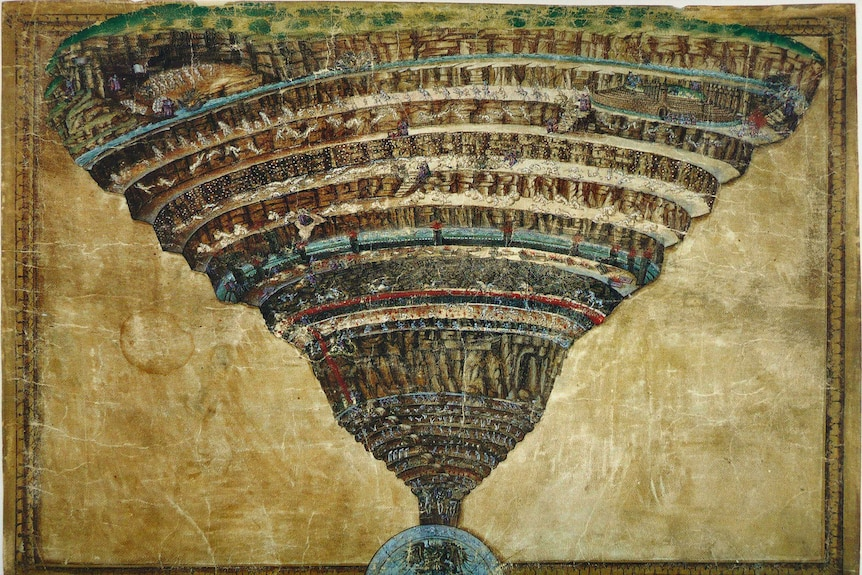
\includegraphics[height=120pt]{assets/Picture_of_Hell.png}
        \captionof{figure}{Hypothesized illustration of Hell}
    \end{center}
    
    但这个子午圈有多宽呢?冰淇淋有多大?
    
    为了证明但丁描述的太阳“与地平线相连”是真实的,伽利略认为诗意意象表明地狱圆顶的直径必须等于地球的半径。
    
    这意味着屋顶的边界将通过法国马赛的西侧和今天的乌兹别克斯坦的塔什干的东侧。
    
    这使得地狱的屋顶成为一个相当大的穹顶——但是,它必须足够大,以容纳现在和将来的居民。
    
    伽利略的下一个问题是计算屋顶的厚度,以防止其坍塌并压垮下面的囚犯。
    
    在这一点上,他又有了一个聪明的想法。伽利略知道佛罗伦萨著名的圣母百花大教堂(今天仍然屹立不倒)宽45米,但只有3米厚。
    
    通过放大比例,他计算出地狱的屋顶必须厚600公里。伽利略最终意识到,这个数字是他计算中的致命错误的产物。但在他注意到之时,他错误的数学描绘地狱的画面已经使他获得了比萨大学的数学讲席。
    
    伽利略没有承认他的错误,也许是为了不失去他的声望和地位,他紧闭双唇,继续思考正确的解决方案。
    
    不过,他在其他事情上可没闷声不响。关于伽利略公开反对教会地球是宇宙中心的观点的故事众所周知,同样众所周知的是这给他惹来了麻烦。
    
    当他在他的《论两大世界系统的对话》中发表他关于日心宇宙的观点时,伽利略犯下了另一个错误。
    
    它采用了对话的形式,其中一个叫Salviati的角色(这就是伽利略自己),一个叫Sagredo的聪明外行(代表现代可能听到RN的人物),以及一个迟钝的回答者叫Simplicio,伽利略关心压制他无思考的观点的人。
    
    伽利略并非完全缺乏政治智慧,他接受了教会当局的指示,将他的日心说称为“假设”,并在他的对话中融入教皇的意见。
    
    他的错误在于把教皇的观点放在Simplicio的口中。伽利略自找麻烦——结果是终身软禁。
    
    在软禁期间,伽利略写了他的另一部著名著作,名为《论两种新科学的对话》。
    
    在这里,他回到了地狱的问题,并最终公开承认了他的第二大错误——地狱穹顶的厚度。
    
    伽利略最初认为屋顶的宽度和厚度可以以相同的方式进行放大——宽度加倍时,他认
    
    为厚度也需要加倍。
    
    那时这是有道理的,但他现在承认自己错了:为了保持结构的强度,厚度必须比宽度更快地增加。
    
    他得出的规则是厚度的立方除以跨度的平方必须保持恒定。
    
    这被称为伽利略的平方立方定律,今天工程师仍在使用。它表明,像梁和屋顶这样的物体在变大时,如果要保持它们的强度,它们必须变得不成比例地更厚。
    
    这甚至适用于动物骨骼,解释了为什么动物的大小存在限制,因为超过一定大小后,它们的骨骼将变得不可能太厚。
    
    它也适用于地狱。当伽利略使用平方立方定律重复他的计算时,他发现屋顶必须如此之厚,以至于几乎没有足够空间容纳所有那些死去的灵魂。
    
    他没有告诉任何人。这可能会让他失去声望和工作。只有在他生命的最后,当他被软禁时,他才把这一切写了下来。
    
    他把地狱及其尺寸的问题转化为现代科学和工程的基础之一。
    
    通过这样做,伽利略确立了一种至今仍然占主导地位的科学方法——坚持将你的信仰与现实相对照。
    
    说到现实:当然,地狱的存在仍然在某些地方存在争议(尽管如果我们使用伽利略的平方立方定律,骨骼能够达到的大小是有限的)。

    \begin{center}
        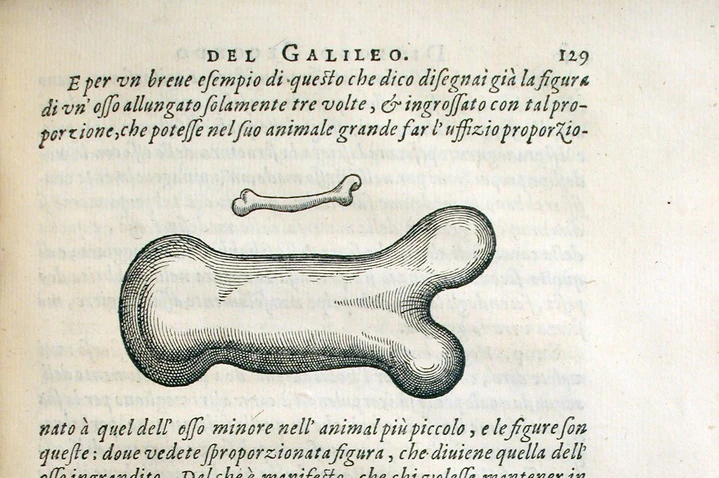
\includegraphics[height=200pt]{assets/The_Bone_in_Square-Cube_law.png}
        \captionof{figure}{The bone in the square-cube law}
    \end{center}
\end{quote}
